% =====================================================================
% 6.1 Convergência
% =====================================================================
\subsection{Convergência}

O ensaio de ordem usa o degrau subamortecido, \(R=20~\Omega\), \(t_f=5~\mathrm{ms}\) e passos de 8~\(\mu\)s a \(0{,}25~\mu\)s. Todos estão abaixo do limite de estabilidade do Euler, que é 20~\(\mu\)s, de modo que a tabela mede ordem e não explosão. A Figura~\ref{fig:conv} mostra o erro máximo da corrente em escala logarítmica. As inclinações seguem 1, 2 e 4.

\begin{table}[htbp]
\centering
\caption{Erro máximo da corrente no degrau subamortecido, em ampères, para \(t\in[0;\,5]~\mathrm{ms}\).}
\label{tab:conv}
\small
\begin{tabular}{@{}rrrr@{}}
\toprule
\(h\) (\(\mu\)s) & Euler & Euler melhorado & RK4 \\
\midrule
8{,}00 & \(9{,}31\times 10^{-3}\) & \(1{,}97\times 10^{-4}\) & \(6{,}32\times 10^{-8}\) \\
4{,}00 & \(4{,}12\times 10^{-3}\) & \(4{,}93\times 10^{-5}\) & \(3{,}94\times 10^{-9}\) \\
2{,}00 & \(1{,}95\times 10^{-3}\) & \(1{,}23\times 10^{-5}\) & \(2{,}46\times 10^{-10}\) \\
1{,}00 & \(9{,}47\times 10^{-4}\) & \(3{,}07\times 10^{-6}\) & \(1{,}53\times 10^{-11}\) \\
0{,}50 & \(4{,}67\times 10^{-4}\) & \(7{,}68\times 10^{-7}\) & \(9{,}58\times 10^{-13}\) \\
0{,}25 & \(2{,}32\times 10^{-4}\) & \(1{,}92\times 10^{-7}\) & \(6{,}00\times 10^{-14}\) \\
\bottomrule
\end{tabular}
\fonte{Elaborado pelo autor (2026).}
\end{table}

A ordem observada entre passos consecutivos, \(\log(E(h)/E(h/2))/\log 2\), aproxima-se de 1{,}010 no Euler, 2{,}000 no Heun e 3{,}996 no RK4 no par mais fino. Um ajuste \(\log E=\log C+p\log h\) em todo o intervalo dá \(p=1{,}060\), \(2{,}001\) e \(4{,}001\). O Euler fica um pouco acima de 1 porque os passos maiores ainda sentem termos de ordem superior; a razão consecutiva já está em 1{,}01. O erro da tensão no capacitor, em volts, permaneceu cerca de cem vezes o erro da corrente, em ampères, em todos os métodos e passos. A razão é a escala das variáveis: \(v_C\) é da ordem de volts e \(i\) da ordem de dezenas de miliampères. A ordem de convergência é a mesma nas duas componentes.

\begin{figure}[htbp]
\centering
\caption{Erro máximo da corrente em função do passo. As retas de referência têm inclinação 1, 2 e 4 e estão ancoradas no maior passo de cada método.}
\label{fig:conv}
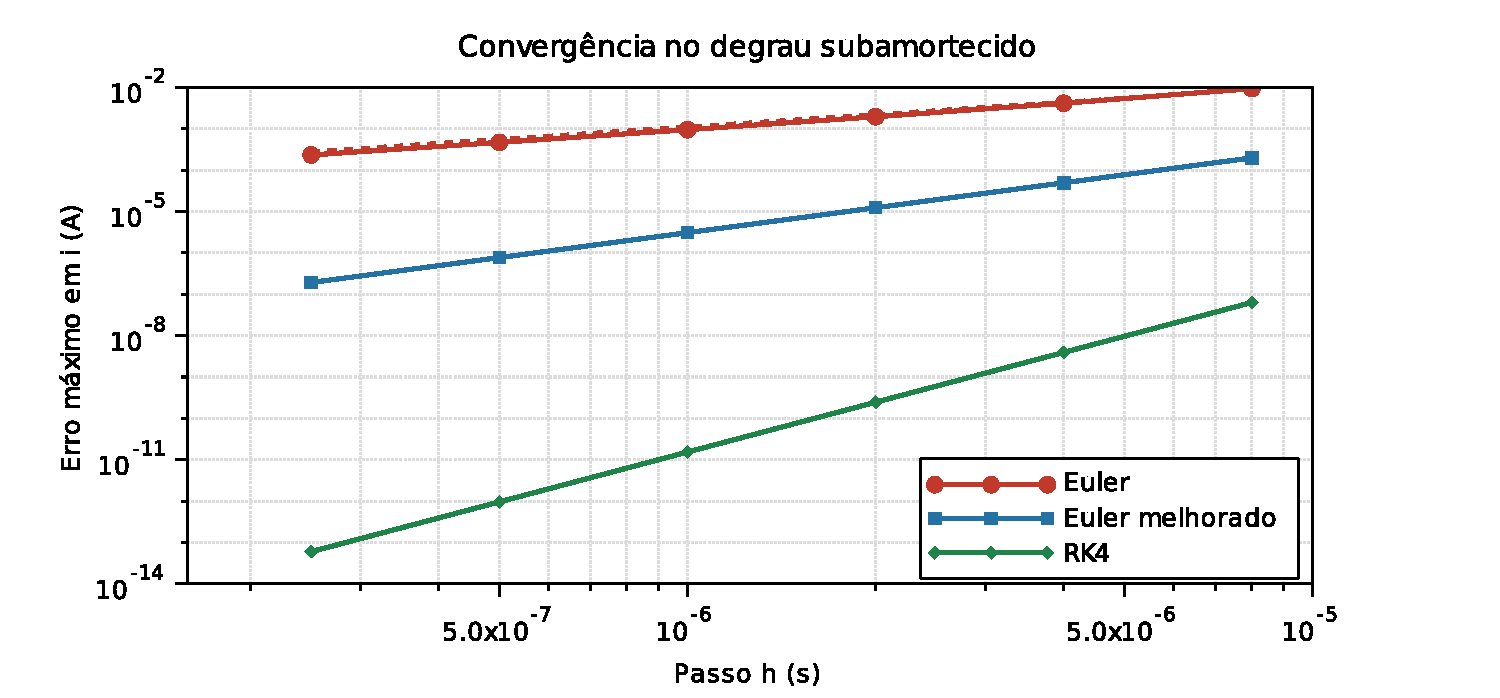
\includegraphics[width=\textwidth]{convergencia.pdf}
\fonte{Elaborado pelo autor (2026).}
\end{figure}

A Figura~\ref{fig:degrau} compara as formas de onda com \(h=15~\mu\mathrm{s}\), ainda estável para o Euler, porém próximo do limite. A solução de Euler oscila por mais tempo do que o circuito: o módulo de \(R(h\lambda)\) é menor do que 1, mas o amortecimento numérico é mais fraco do que \(\alpha\). Heun e RK4 sobrepõem-se à solução analítica nessa escala. A Figura~\ref{fig:erro} separa os três erros. Com \(h=8~\mu\mathrm{s}\), o erro de pico do Euler é da ordem de \(10^{-2}\)~A; o do Heun, de \(10^{-4}\)~A; o do RK4, de \(10^{-8}\)~A. Reduzir o passo a \(2~\mu\mathrm{s}\) divide o erro do Euler por cerca de quatro, o do Heun por cerca de dezesseis e o do RK4 por cerca de duzentos e cinquenta, de novo as potências de \(2^{p}\).

\begin{figure}[htbp]
\centering
\caption{Resposta ao degrau de 5~V com \(R=20~\Omega\) e \(h=15~\mu\mathrm{s}\). Euler ainda é estável, mas o amortecimento numérico é visivelmente menor do que o do circuito.}
\label{fig:degrau}
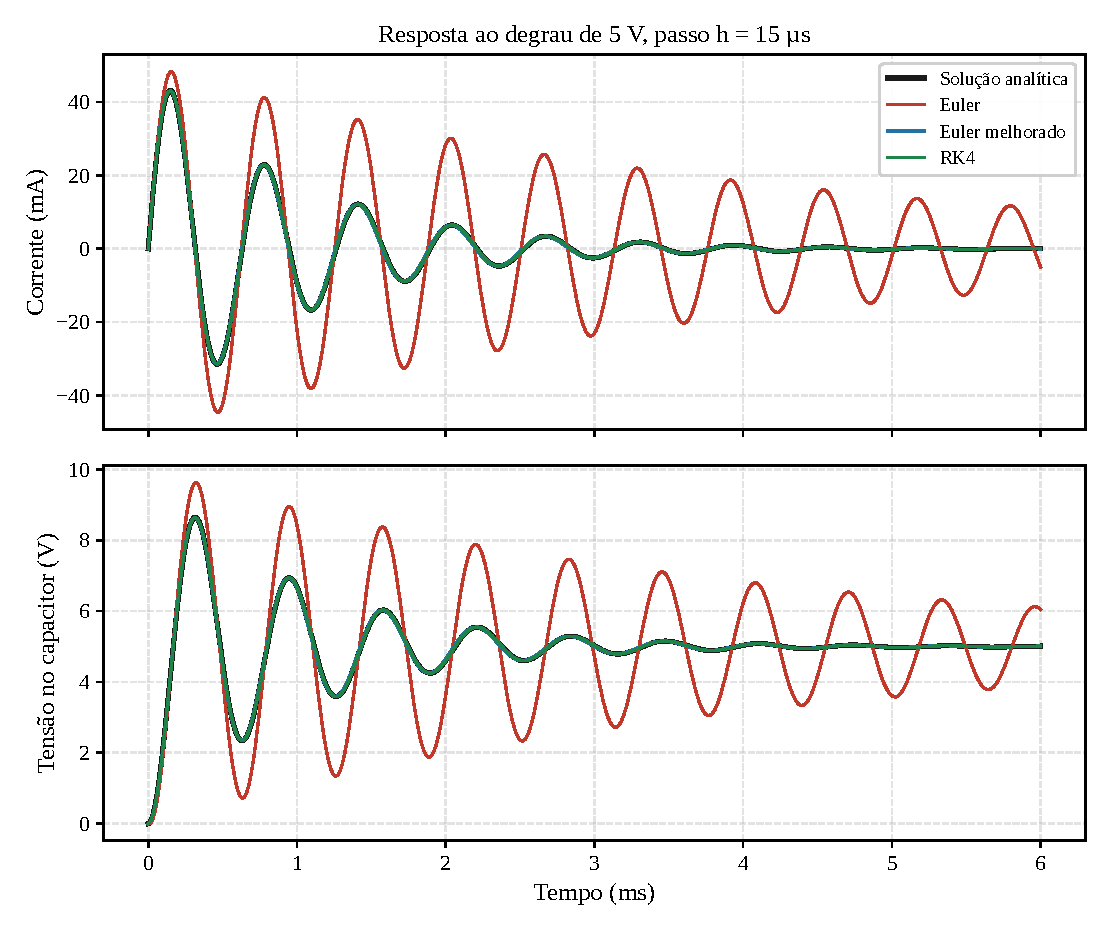
\includegraphics[width=\textwidth]{resposta_degrau.pdf}
\fonte{Elaborado pelo autor (2026).}
\end{figure}

\begin{figure}[htbp]
\centering
\caption{Erro absoluto da corrente ao longo do tempo, nos passos de 8~\(\mu\)s e de 2~\(\mu\)s. A oscilação do erro acompanha a corrente do circuito.}
\label{fig:erro}
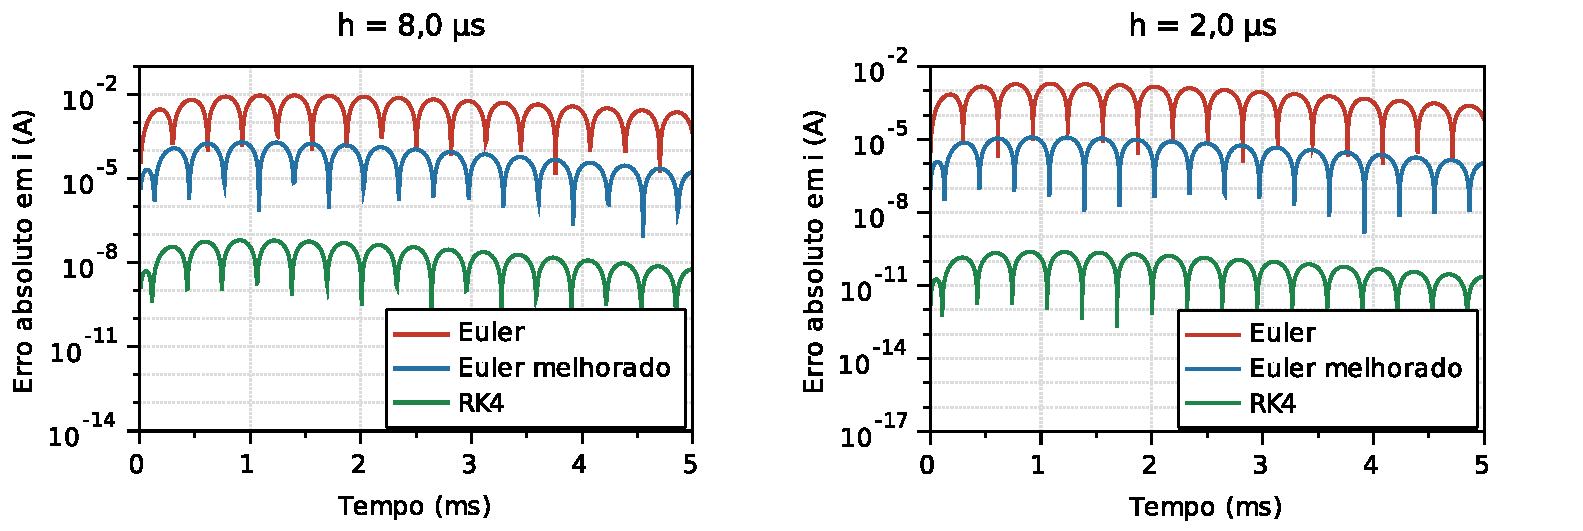
\includegraphics[width=\textwidth]{erro_temporal.pdf}
\fonte{Elaborado pelo autor (2026).}
\end{figure}
